%%%%%%%%%%%%%%%%%%%%%%%%%%%%%%%%%%%%%%%%%%%%%%%%%%%%%%%%%%%%%%%%%%
%
% Analysis of Algorithms
%
% Homework Assignment #6
%
%%%%%%%%%%%%%%%%%%%%%%%%%%%%%%%%%%%%%%%%%%%%%%%%%%%%%%%%%%%%%%%%%%
%%%%%%%%%%%%%%%%%%%%%%%%%%%%%%%%%%%%%%%%%%%%%%%%%%%%%%%%%%%%%%%%%%
%
% Score Card and Answer Sheets
%
%%%%%%%%%%%%%%%%%%%%%%%%%%%%%%%%%%%%%%%%%%%%%%%%%%%%%%%%%%%%%%%%%%
\documentclass[addpoints,11pt]{exam}
\usepackage{amsmath}
\usepackage{amstext}
\usepackage{clrscode3e}
\usepackage{enumitem}
\usepackage{fullpage}
\usepackage{xcolor}
\usepackage{minted}
\usepackage{graphicx}
\usepackage{float}

%%%%%%%%%%%%%%%%%%%%%%%%%%%%%%%%%%%%%%%%%%%%%%%%%%%%%%%%%%%%%%%%%%
%
% Begin Document
%
%%%%%%%%%%%%%%%%%%%%%%%%%%%%%%%%%%%%%%%%%%%%%%%%%%%%%%%%%%%%%%%%%%
\begin{document}
\pagestyle{empty}


\noindent{\large\bfseries Name: \hrulefill John Henry Mejia}\\
\noindent{\large\bfseries COSC 40403 - Analysis of Algorithms: Homework 6}\\
\noindent{\large\bfseries Due: 10:59 on November 29}


%%%%%%%%%%%%%%%%%%%%%%%%%%%%%%%%%%%%%%%%%%%%%%%%%%%%%%%%%%%%%%%%%%
%
% Score Card and Answer Sheets
%
% Comment out one-or-the-other to show or not-show the answers.
%
%%%%%%%%%%%%%%%%%%%%%%%%%%%%%%%%%%%%%%%%%%%%%%%%%%%%%%%%%%%%%%%%%%
%\SolutionEmphasis{\color{violet}}

\renewcommand{\solutiontitle}{\noindent\textbf{Answer:}\par\noindent}

\printanswers
%%\noprintanswers



%%%%%%%%%%%%%%%%%%%%%%%%%%%%%%%%%%%%%%%%%%%%%%%%%%%%%%%%%%%%%%%%%%
% Begin Questions
%%%%%%%%%%%%%%%%%%%%%%%%%%%%%%%%%%%%%%%%%%%%%%%%%%%%%%%%%%%%%%%%%%
\begin{questions}


%%%%%%%%%%%%%%%%%%%%%%%%%%%%%%%%%%%%%%%%%%%%%%%%%%%%%%%%%%%%%%%%%%
% Question
%%%%%%%%%%%%%%%%%%%%%%%%%%%%%%%%%%%%%%%%%%%%%%%%%%%%%%%%%%%%%%%%%%
\question[5]
Modify $\proc{Memoized-Cut-Rod}$ to return not only the value but the actual solution.

\begin{solutionorbox}
\begin{minted}{python}
def memoized_cut_rod(p, n):
    r = []
    s = []
    for i in range(0, n + 1):
        r.append(-1)
        s.append(0)
    memoized_cut_rod_aux(p, n, r, s)
    return r[n], s

def memoized_cut_rod_aux(p, n, r, s):
    if r[n] >= 0:
        return r[n]
    if n == 0:
        q = 0
    else:
        q = -1
        for i in range(1, n + 1):
            if q < p[i] + memoized_cut_rod_aux(p, n - i, r, s):
                q = p[i] + memoized_cut_rod_aux(p, n - i, r, s)
                s[n] = i
    r[n] = q
    return q

#Example of how to use the memoized_cut_rod function
p = [0, 1, 5, 8, 9, 10, 17, 17, 20, 24, 30]
n = 4
print (memoized_cut_rod(p, n))

\end{minted}
\end{solutionorbox}

\ifprintanswers
\newpage
\else
\bigskip
\fi


%%%%%%%%%%%%%%%%%%%%%%%%%%%%%%%%%%%%%%%%%%%%%%%%%%%%%%%%%%%%%%%%%%
% Question
%%%%%%%%%%%%%%%%%%%%%%%%%%%%%%%%%%%%%%%%%%%%%%%%%%%%%%%%%%%%%%%%%%
\question[5]
Consider a modification of the rod-cutting problem in which, in addition to a price $p_i$ for each rod, each cut incurs a fixed cost of $c$.  The revenue associated with a solution is now the sum of the prices of the pieces minus the costs of making the cuts.  Give a dynamic-programming algorithm (similar to what was presented in lecture) to solve this modified problem.  Be sure to also explain you answer.

\begin{solutionorbox}
\begin{codebox}
    \li //Size of the rod, price table, cost per cut
	\Procname{$\proc{Cut-Rod-Cost}(n, P, c)$}
        \li $r$ = $[]$ // New array of size 0-n
        \li r[0] = 0
        \li \For $(i = 1; i < n; i++)$ \Do
	\li q = p[i]
        \li \For $(j = 1; j < i-1; j++)$ \Do
        \li q = \proc{max} $( q , p [ j ] + r \cdot [ i - j  ]$ - $ c )$ //Subtract the cost

        
	\End
        \li r[i] = q
	\End
        \li return $r[n]$
    \end{codebox}



    Generally, it is the same as algorithm as before. However, the revenue takes into account the cost; that is, the updated revenue is: price of the left piece + optimal price of the rest of the rod - cost of cut. 
    \begin{itemize}
        \item Something to keep in mind is that if we don't add a cut then there's 0 cost of cut. (no need to update that case)
    \end{itemize} 
\end{solutionorbox}

\ifprintanswers
\newpage
\else
\bigskip
\fi


%%%%%%%%%%%%%%%%%%%%%%%%%%%%%%%%%%%%%%%%%%%%%%%%%%%%%%%%%%%%%%%%%%
% Question
%%%%%%%%%%%%%%%%%%%%%%%%%%%%%%%%%%%%%%%%%%%%%%%%%%%%%%%%%%%%%%%%%%
\question [10]
Find the optimal order, and its cost, for evaluating the product $A_1 \times A_2 \times A_3 \times A_4 \times A_5$ where
\begin{enumerate}
	\item $A_1$ is $(10 \times 4)$
	\item $A_2$ is $(4 \times 5)$
	\item $A_3$ is $(5 \times 20)$
	\item $A_4$ is $(20 \times 2)$
	\item $A_5$ is $(2 \times 50)$
\end{enumerate}
Show your work for partial credit.

\begin{solutionorbox}
RECALL: Matrices are found in row x column fashion.

When you multiply 2 matrices the resulting matrix C found by multiplying the matrices [A1, A2] and [B1, B2] (that is, A x B)  will be of dimensions [A1, B2]. 

Therefore there will be $A1 \cdot B2$ elements there, and for each element you must do $A2 \cdot B1$ multiplications to get it. (the number of multiplications is the cost.)

There are 42 possible ways to do this specific problem: $\frac{{(2n) \choose n}}{n+1} $

\begin{table}[H]
\begin{tabular}{llllll}
M & 1 & 2   & 3    & 4   & 5    \\
1 & 0 & 200 & 1200 & 320 & 1320 \\
2 &   & 0   & 400  & 240 & 640  \\
3 &   &     & 0    & 200 & 700  \\
4 &   &     &      & 0   & 2000 \\
5 &   &     &      &     & 0   
\end{tabular}
\end{table}

Our solution is 

$(A_1(A_2(A_3 \times A_4))) \times A_5$

Total cost: 

$A_3 \times A_4 = 5 \cdot 2 \cdot 20 = $ cost of 200

$A_2 \times A_4 A_3 = 4 \cdot 5 \cdot 2 = $ cost of 40 + 200 = 240 total 

$A_1 \times A_4 A_3 A_2 = 10 \cdot 4 \cdot 2 = $ cost of 80 + 240 = 320 total 

$A_5 \times A_4 A_3 A_2 A_1 = 10 \cdot 2 \cdot 50 = $ cost of 1000 + 320 = 1320 total 

The minimum cost is 1320

\end{solutionorbox}

\ifprintanswers
\newpage
\else
\bigskip
\fi


%%%%%%%%%%%%%%%%%%%%%%%%%%%%%%%%%%%%%%%%%%%%%%%%%%%%%%%%%%%%%%%%%%
% Question
%%%%%%%%%%%%%%%%%%%%%%%%%%%%%%%%%%%%%%%%%%%%%%%%%%%%%%%%%%%%%%%%%%
\question[15]
Determine the LCS of $\langle 1, 0, 0, 1, 0, 1, 0, 1 \rangle$ and $\langle 0, 1, 0, 1, 1, 0, 1, 1, 0 \rangle$.  Show your work for partial credit.

\begin{solutionorbox}

The LCS is 010101, that is, a length of 6. 


\begin{minted}{python}
def lcs(X, Y):
    m = len(X)
    n = len(Y)
    L = [[0 for x in range(n+1)] for x in range(m+1)]
    for i in range(m+1):
        for j in range(n+1):
            if i == 0 or j == 0:
                L[i][j] = 0
            elif X[i-1] == Y[j-1]:
                L[i][j] = L[i-1][j-1] + 1
            else:
                L[i][j] = max(L[i-1][j], L[i][j-1])
    index = L[m][n]
    lcs = [""] * (index+1)
    lcs[index] = ""
    i = m
    j = n
    while i > 0 and j > 0:
        if X[i-1] == Y[j-1]:
            lcs[index-1] = X[i-1]
            i -= 1
            j -= 1
            index -= 1
        elif L[i-1][j] > L[i][j-1]:
            i -= 1
        else:
            j -= 1
    return lcs[0:-1]
\end{minted}

Work: 

Let us refer to the first list as list X and the 2nd list as list Y. 

The naive way is, of course, to generate all common subsequences and pick the longest one. However, using dynamic programming, we can do better. 

We create a table of dimension n+1*m+1 where n and m are the lengths of X and Y respectively. The first row and the first column are filled with zeros.
If the character corresponding to the current row and current column are matching, then fill the current cell by adding one to the diagonal element. Point an arrow to the diagonal cell.
Else take the maximum value from the previous column and previous row element for filling the current cell. Point an arrow to the cell with maximum value. If they are equal, point to any of them.

If you follow the logic then there is the table shown below ! 

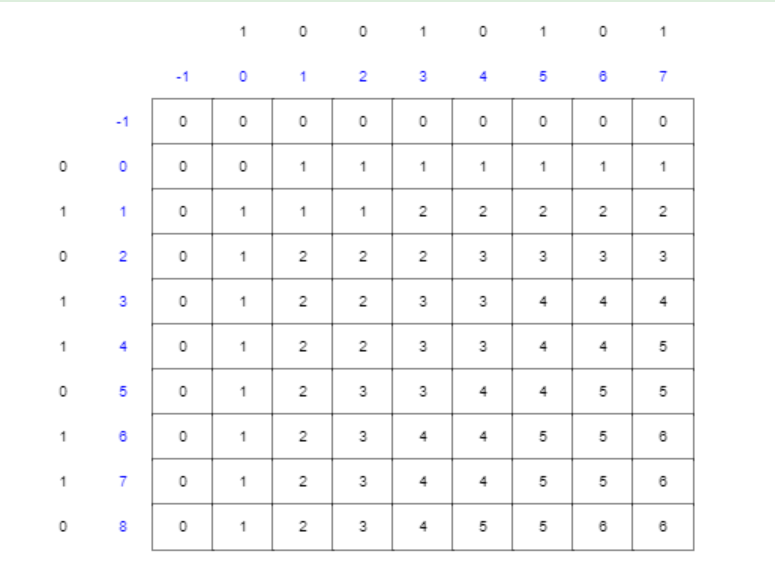
\includegraphics{image.png}

Then we just follow the path of diagonals to get the longest subsequence! 

010101

\end{solutionorbox}

\ifprintanswers
\newpage
\else
\bigskip
\fi


%%%%%%%%%%%%%%%%%%%%%%%%%%%%%%%%%%%%%%%%%%%%%%%%%%%%%%%%%%%%%%%%%%
% Question
%%%%%%%%%%%%%%%%%%%%%%%%%%%%%%%%%%%%%%%%%%%%%%%%%%%%%%%%%%%%%%%%%%
\question[25]
The \textbf{\textit{Moneyball}} Problem.  Suppose you are the GM for a professional sports team.  You need to sign some free-agent players to your team during the off season.  The owner of the team has given you \$$X$ to spend on free agents.  You can spend less than \$$X$ but not any more.\\

You would like to fill $N$ different positions on your team.  Each position has $P$ free-agent players who are available.  Because you do not want to overload your roster with too many players at any one position, for each position you may sign at most one free agent who plays that position.  If you do not sign any players at a particular position, then you plan to stick with the players you already have at that position.\\

To determine how valuable a player is going to be, you decide to use the a metric called ``profit above replacement'' (PAR).  A player with a higher PAR is more valuable than a player with a lower PAR.  A player with a higher PAR is not necessarily more expensive to sign than a player with a lower PAR, because factors other than a player's value determine how must it costs to sign him.\\

For each available free-agent player, you have three pieces of information.
\begin{enumerate}
	\item the player's position
	\item the amount of money it will cost to sign the player
	\item the player's PAR
\end{enumerate} 

Devise an algorithm that maximizes the total PAR of the players you sign while spending no more than \$$X$ dollars.  You may assume that each player signs for a multiple of \$50,000.  Your algorithm should output the total PAR of the players you sign, the total amount of money you spend, and a list of which players you sign.  Analyze the running time and space of your algorithm (using dynamic programming...of course). \\

\textbf{Make sure you follow the four step process of dynamic programming.}


\begin{solutionorbox}

This is essentially a extension of the bounded knapsack problem- you are attempting to maximize the PAR with your budget However, the difference from the unbounded version is that you can only have one free agent per position.

The 4 steps of dynamic programming are: 
\begin{itemize}
    \item Characterize the structure of an optimal solution.
    \item Recursively define the value of an optimal solution.
    \item Compute the value of an optimal solution, typically in a bottom-up fashion.
    \item Construct an optimal solution from the computed information.
\end{itemize}

Our solution should be of the following fashion: a matrix of length N (one for each position), where each position has either a given player, or a blank player (ie. no change, costing \$0, but with a PAR of 0.) 

From there we can get the Total PAR of the players we sign, the total amount of money we spend, and a list of which players we sign.

\begin{codebox}
    \li //number of positions, budget, playerlist
	\Procname{$\proc{MoneyBall}(N, X, P)$}

    \li initialize a table B of size (N + 1) by (X + 1)
    \li initialize an array P of length N
    \li \For i = 0 to N \Do
        \li B[i, 0] = 0
    \End
    \li \For j = 1 to X \Do
        \li B[0, j] = 0
    \End
    \li \For i = 1 to N \Do
        \li \For j = 1 to X \Do
            \li \If j $<$ i.cost \Do
                \li B[i, j] = B[i - 1, j]
                \End
            \li q = B[i - 1, j]
            \li p = 0
            \li \For k = 1 to P \Do
                \li \If j $>$= i.cost \Do
                    \li t = B[i - 1, j - i.cost] + i.value
                    \li \If t $>$ q \Do
                        \li q = t
                        \li p = k
                    \End
                    \End
                    \End
            \li B[i, j] = q
            \li P[i] = p
            \End
            \End
    \li print("The total PAR is " + B[N, X] + " and the players are:")
    \li i = N
    \li j = X
    \li C = 0
    \li \For k = 1 to N \Do
        \li \If B[i, j] != B[i - 1, j] \Do
        \li print(P[i])
            \li j = j - i.cost
            \li C = C + i.cost
            \End
        \li i = i - 1
        \End
    \li print("The total cost is" + C)

    \end{codebox}


Since each player signs for a multiple for \$50,000 then I would start by doing some.

The running time is the O(number of positions $\cdot$ number of players available)

The space complexity is O(number of positions $\cdot$ number of players avaialable)
\end{solutionorbox}


%%%%%%%%%%%%%%%%%%%%%%%%%%%%%%%%%%%%%%%%%%%%%%%%%%%%%%%%%%%%%%%%%%
%%%%%%%%%%%%%%%%%%%%%%%%%%%%%%%%%%%%%%%%%%%%%%%%%%%%%%%%%%%%%%%%%%
\end{questions}


%%%%%%%%%%%%%%%%%%%%%%%%%%%%%%%%%%%%%%%%%%%%%%%%%%%%%%%%%%%%%%%%%%
%%%%%%%%%%%%%%%%%%%%%%%%%%%%%%%%%%%%%%%%%%%%%%%%%%%%%%%%%%%%%%%%%%
\end{document}
